\documentclass{ximera}

%\usepackage{todonotes}

\newcommand{\todo}{}

\usepackage{esint} % for \oiint
\ifxake%%https://math.meta.stackexchange.com/questions/9973/how-do-you-render-a-closed-surface-double-integral
\renewcommand{\oiint}{{\large\bigcirc}\kern-1.56em\iint}
\fi


\graphicspath{
  {./}
  {ximeraTutorial/}
  {basicPhilosophy/}
  {functionsOfSeveralVariables/}
  {normalVectors/}
  {lagrangeMultipliers/}
  {vectorFields/}
  {greensTheorem/}
  {shapeOfThingsToCome/}
  {dotProducts/}
  {partialDerivativesAndTheGradientVector/}
  {../productAndQuotientRules/exercises/}
  {../normalVectors/exercisesParametricPlots/}
  {../continuityOfFunctionsOfSeveralVariables/exercises/}
  {../partialDerivativesAndTheGradientVector/exercises/}
  {../directionalDerivativeAndChainRule/exercises/}
  {../commonCoordinates/exercisesCylindricalCoordinates/}
  {../commonCoordinates/exercisesSphericalCoordinates/}
  {../greensTheorem/exercisesCurlAndLineIntegrals/}
  {../greensTheorem/exercisesDivergenceAndLineIntegrals/}
  {../shapeOfThingsToCome/exercisesDivergenceTheorem/}
  {../greensTheorem/}
  {../shapeOfThingsToCome/}
  {../separableDifferentialEquations/exercises/}
  {vectorFields/}
}

\newcommand{\mooculus}{\textsf{\textbf{MOOC}\textnormal{\textsf{ULUS}}}}

\usepackage{tkz-euclide}
\usepackage{tikz}
\usepackage{tikz-cd}
\usetikzlibrary{arrows}
\tikzset{>=stealth,commutative diagrams/.cd,
  arrow style=tikz,diagrams={>=stealth}} %% cool arrow head
\tikzset{shorten <>/.style={ shorten >=#1, shorten <=#1 } } %% allows shorter vectors

\usetikzlibrary{backgrounds} %% for boxes around graphs
\usetikzlibrary{shapes,positioning}  %% Clouds and stars
\usetikzlibrary{matrix} %% for matrix
\usepgfplotslibrary{polar} %% for polar plots
\usepgfplotslibrary{fillbetween} %% to shade area between curves in TikZ
%\usetkzobj{all}
\usepackage[makeroom]{cancel} %% for strike outs
%\usepackage{mathtools} %% for pretty underbrace % Breaks Ximera
%\usepackage{multicol}
\usepackage{pgffor} %% required for integral for loops



%% http://tex.stackexchange.com/questions/66490/drawing-a-tikz-arc-specifying-the-center
%% Draws beach ball
\tikzset{pics/carc/.style args={#1:#2:#3}{code={\draw[pic actions] (#1:#3) arc(#1:#2:#3);}}}



\usepackage{array}
\setlength{\extrarowheight}{+.1cm}
\newdimen\digitwidth
\settowidth\digitwidth{9}
\def\divrule#1#2{
\noalign{\moveright#1\digitwidth
\vbox{\hrule width#2\digitwidth}}}




% \newcommand{\RR}{\mathbb R}
% \newcommand{\R}{\mathbb R}
% \newcommand{\N}{\mathbb N}
% \newcommand{\Z}{\mathbb Z}

\newcommand{\sagemath}{\textsf{SageMath}}


%\renewcommand{\d}{\,d\!}
%\renewcommand{\d}{\mathop{}\!d}
%\newcommand{\dd}[2][]{\frac{\d #1}{\d #2}}
%\newcommand{\pp}[2][]{\frac{\partial #1}{\partial #2}}
% \renewcommand{\l}{\ell}
%\newcommand{\ddx}{\frac{d}{\d x}}

% \newcommand{\zeroOverZero}{\ensuremath{\boldsymbol{\tfrac{0}{0}}}}
%\newcommand{\inftyOverInfty}{\ensuremath{\boldsymbol{\tfrac{\infty}{\infty}}}}
%\newcommand{\zeroOverInfty}{\ensuremath{\boldsymbol{\tfrac{0}{\infty}}}}
%\newcommand{\zeroTimesInfty}{\ensuremath{\small\boldsymbol{0\cdot \infty}}}
%\newcommand{\inftyMinusInfty}{\ensuremath{\small\boldsymbol{\infty - \infty}}}
%\newcommand{\oneToInfty}{\ensuremath{\boldsymbol{1^\infty}}}
%\newcommand{\zeroToZero}{\ensuremath{\boldsymbol{0^0}}}
%\newcommand{\inftyToZero}{\ensuremath{\boldsymbol{\infty^0}}}



% \newcommand{\numOverZero}{\ensuremath{\boldsymbol{\tfrac{\#}{0}}}}
% \newcommand{\dfn}{\textbf}
% \newcommand{\unit}{\,\mathrm}
% \newcommand{\unit}{\mathop{}\!\mathrm}
% \newcommand{\eval}[1]{\bigg[ #1 \bigg]}
% \newcommand{\seq}[1]{\left( #1 \right)}
% \renewcommand{\epsilon}{\varepsilon}
% \renewcommand{\phi}{\varphi}


% \renewcommand{\iff}{\Leftrightarrow}

% \DeclareMathOperator{\arccot}{arccot}
% \DeclareMathOperator{\arcsec}{arcsec}
% \DeclareMathOperator{\arccsc}{arccsc}
% \DeclareMathOperator{\si}{Si}
% \DeclareMathOperator{\scal}{scal}
% \DeclareMathOperator{\sign}{sign}


%% \newcommand{\tightoverset}[2]{% for arrow vec
%%   \mathop{#2}\limits^{\vbox to -.5ex{\kern-0.75ex\hbox{$#1$}\vss}}}
% \newcommand{\arrowvec}[1]{{\overset{\rightharpoonup}{#1}}}
% \renewcommand{\vec}[1]{\arrowvec{\mathbf{#1}}}
% \renewcommand{\vec}[1]{{\overset{\boldsymbol{\rightharpoonup}}{\mathbf{#1}}}}

% \newcommand{\point}[1]{\left(#1\right)} %this allows \vector{ to be changed to \vector{ with a quick find and replace
% \newcommand{\pt}[1]{\mathbf{#1}} %this allows \vec{ to be changed to \vec{ with a quick find and replace
% \newcommand{\Lim}[2]{\lim_{\point{#1} \to \point{#2}}} %Bart, I changed this to point since I want to use it.  It runs through both of the exercise and exerciseE files in limits section, which is why it was in each document to start with.

% \DeclareMathOperator{\proj}{\mathbf{proj}}
% \newcommand{\veci}{{\boldsymbol{\hat{\imath}}}}
% \newcommand{\vecj}{{\boldsymbol{\hat{\jmath}}}}
% \newcommand{\veck}{{\boldsymbol{\hat{k}}}}
% \newcommand{\vecl}{\vec{\boldsymbol{\l}}}
% \newcommand{\uvec}[1]{\mathbf{\hat{#1}}}
% \newcommand{\utan}{\mathbf{\hat{t}}}
% \newcommand{\unormal}{\mathbf{\hat{n}}}
% \newcommand{\ubinormal}{\mathbf{\hat{b}}}

% \newcommand{\dotp}{\bullet}
% \newcommand{\cross}{\boldsymbol\times}
% \newcommand{\grad}{\boldsymbol\nabla}
% \newcommand{\divergence}{\grad\dotp}
% \newcommand{\curl}{\grad\cross}
%\DeclareMathOperator{\divergence}{divergence}
%\DeclareMathOperator{\curl}[1]{\grad\cross #1}
% \newcommand{\lto}{\mathop{\longrightarrow\,}\limits}

% \renewcommand{\bar}{\overline}

\colorlet{textColor}{black}
\colorlet{background}{white}
\colorlet{penColor}{blue!50!black} % Color of a curve in a plot
\colorlet{penColor2}{red!50!black}% Color of a curve in a plot
\colorlet{penColor3}{red!50!blue} % Color of a curve in a plot
\colorlet{penColor4}{green!50!black} % Color of a curve in a plot
\colorlet{penColor5}{orange!80!black} % Color of a curve in a plot
\colorlet{penColor6}{yellow!70!black} % Color of a curve in a plot
\colorlet{fill1}{penColor!20} % Color of fill in a plot
\colorlet{fill2}{penColor2!20} % Color of fill in a plot
\colorlet{fillp}{fill1} % Color of positive area
\colorlet{filln}{penColor2!20} % Color of negative area
\colorlet{fill3}{penColor3!20} % Fill
\colorlet{fill4}{penColor4!20} % Fill
\colorlet{fill5}{penColor5!20} % Fill
\colorlet{gridColor}{gray!50} % Color of grid in a plot

\newcommand{\surfaceColor}{violet}
\newcommand{\surfaceColorTwo}{redyellow}
\newcommand{\sliceColor}{greenyellow}




\pgfmathdeclarefunction{gauss}{2}{% gives gaussian
  \pgfmathparse{1/(#2*sqrt(2*pi))*exp(-((x-#1)^2)/(2*#2^2))}%
}


%%%%%%%%%%%%%
%% Vectors
%%%%%%%%%%%%%

%% Simple horiz vectors
\renewcommand{\vector}[1]{\left\langle #1\right\rangle}


%% %% Complex Horiz Vectors with angle brackets
%% \makeatletter
%% \renewcommand{\vector}[2][ , ]{\left\langle%
%%   \def\nextitem{\def\nextitem{#1}}%
%%   \@for \el:=#2\do{\nextitem\el}\right\rangle%
%% }
%% \makeatother

%% %% Vertical Vectors
%% \def\vector#1{\begin{bmatrix}\vecListA#1,,\end{bmatrix}}
%% \def\vecListA#1,{\if,#1,\else #1\cr \expandafter \vecListA \fi}

%%%%%%%%%%%%%
%% End of vectors
%%%%%%%%%%%%%

%\newcommand{\fullwidth}{}
%\newcommand{\normalwidth}{}



%% makes a snazzy t-chart for evaluating functions
%\newenvironment{tchart}{\rowcolors{2}{}{background!90!textColor}\array}{\endarray}

%%This is to help with formatting on future title pages.
\newenvironment{sectionOutcomes}{}{}



%% Flowchart stuff
%\tikzstyle{startstop} = [rectangle, rounded corners, minimum width=3cm, minimum height=1cm,text centered, draw=black]
%\tikzstyle{question} = [rectangle, minimum width=3cm, minimum height=1cm, text centered, draw=black]
%\tikzstyle{decision} = [trapezium, trapezium left angle=70, trapezium right angle=110, minimum width=3cm, minimum height=1cm, text centered, draw=black]
%\tikzstyle{question} = [rectangle, rounded corners, minimum width=3cm, minimum height=1cm,text centered, draw=black]
%\tikzstyle{process} = [rectangle, minimum width=3cm, minimum height=1cm, text centered, draw=black]
%\tikzstyle{decision} = [trapezium, trapezium left angle=70, trapezium right angle=110, minimum width=3cm, minimum height=1cm, text centered, draw=black]


\title{Gravity}

\begin{document}

\begin{abstract}
inverse square law
\end{abstract}
\maketitle




Gravity affects the trajectory of every projectile.  Gravity is a force and pulls objects down to the Earth. This force is greater on objects with more mass and weaker the farther the objects are from the Earth.




\subsection*{Newton}

Newton's law of gravitation is an inverse square law

\[ F_g = \frac{G \, m_1 \, m_2}{r^2}    \]




where $G = 6.67 \times 10^{-11} \frac{m^3}{kg \cdot s^2}$ is the gravitational constant. \\


$F_g$ is the gravitational force between point-masses $m_1$ and $m_2$, which are a distance $r$ apart. \\


For us:
\begin{itemize}
\item the two masses are our projectile ($m_p$) and the Earth ($m_e$).
\item $r$ is the distance between the centers of our masses. Our projectiles are a negligent distance off of the Earth.  Therefore, we can just say that $r = r_e$ (the radius of the Earth).  $r$ is basically just a constant for us.
\end{itemize}



Now, add in the fact that $F = m \, a$ and this tells us that the gravity(acceleration) a projectile feels from the Earth is given by


\[ g = \frac{F_g}{m_p}  = \frac{G \, m_e}{(r_e)^2}    \]


\[ g = \frac{(6.67 \times 10^{-11} \frac{m^3}{kg \cdot s^2}) \cdot (5.972 \times 10^{24} \, kg)}{(6356 \, km)^2} = 9.81 \frac{m}{s^2}   \]


A constant! \\

This is the acceleration we feel on Earth, a downward acceleration, $-9.81 \frac{m}{s^2}$.   That means, for most of our investigations, the acceleration due to the Earth can be considered a constant.




$\blacktriangleright$ Gravity is constant acceleration.

The acceleration due to the Earth's gravity is a constant.  It is a constant function with respect to time or position.


\[ a(t) = -9.81 \, \frac{m}{s^2}  \]



Acceleration is meters per second PER second.  This constant acceleration is a constant rate of change of velocity.  Thus, vertical velocity must be a linear function.




\[ v(t) = v_0 - 9.81 \, t  \, \frac{m}{s}\]



This velocity is a linear function. The accumulated vertical distance traveled would be the accumulated area under its graph. We have seen that this area (distance) is a described by a quadratic. 




\[ h(t) = s_0 + v_0 \, t - \frac{9.81}{2} \, t^2  \]




\begin{itemize}
\item $v_0$ is the initial (vertical) velocity for a projectile thrown into the air. \\

\item $s_0$ is the initial height for a projectile thrown into the air. \\

\item $h(t)$ is height (vertical distance) as a function of time.  Seconds is the domain unit and meters is the range unit.
\end{itemize}



\begin{summary} Projectiles



$\blacktriangleright$ Acceleration due to the Earth is a \wordChoice{\choice[correct]{constant} \choice{linear} \choice{quadratic}}. \\

$\blacktriangleright$ Acceleration is the rate of change of velocity, which makes velocity \wordChoice{\choice{constant} \choice[correct]{linear} \choice{quadratic}}. \\

$\blacktriangleright$ The area under the velocity graph measures the distance traveled, which makes this area \wordChoice{\choice{constant} \choice{linear} \choice[correct]{quadratic}}. \\

$\blacktriangleright$ Distance traveled is a \wordChoice{\choice{constant} \choice{linear} \choice[correct]{quadratic}}. \\




\begin{quote}
\begin{itemize}
\item The rate of change of a quadratic is linear.
\item The rate of change of a linear is constant.
\end{itemize}
\end{quote}



\end{summary}








\subsection*{Projectile Motion}


Actually, all of those quantities are vectors.  They are actually holding two pieces of information simultaneously. They are holding a vertical measurement and a horizontal measurement. \\

\begin{observation}
For a projectile thrown into the air, 
\begin{itemize}
\item There is a vertical position, a vertical velocity, and a vertical acceleration
\item There is a horizontal position, a horizontal velocity, and a horizontal acceleration
\end{itemize}
\end{observation}



Both the vertical, $y$, and horizontal, $x$, components of position are functions of time.

We have already seen this equation for the height (vertical distance) of a projectile.

\[ 
D_y(t) = s_{y_0} + v_{y_0} \, t - \frac{9.81}{2} t^2  
\]

Horizontal motion isn't effected by the Earth's gravity, since gravity is a downward acceleration. Therefore, the horizontal distance is just affected by the initial horizontal velocity.


\[ 
D_x(t) = s_{x_0} + v_{x_0} \, t  
\]






\begin{definition} \textbf{\textcolor{green!50!black}{Parameterization}} \\

The flight path through the air of an object thrown at an angle is a parabola.  This parabola is the graph of a function containing pairs of the form $(horizontal \, distance, vertical \,distance)$ \\

In the discussion above, we separated these two distance measurements into separate functions where the domain for each became time.



When we separate two related measurements and describe each by itself compared to a common third measurement, we call this process \textbf{parameterization}.  The resulting two functions together are called the \textbf{parameterization}.  The new third measurement is called the \textbf{parameter}.





\begin{model} 


The Parameterized Model for projectile motion is


\begin{itemize}
\item $D_x(t) = s_{x_0} + v_{x_0} t$
\item $D_y(t) = s_{y_0} + v_{y_0} t - \frac{9.81}{2} t^2$
\end{itemize}

$t$ is the parameter.

\end{model}



\end{definition}

















\subsection*{Parabolas}

Parabolas are geometric curves.  They are defined as the collection of points which are equidistant from a point, called the \textbf{focus}, and a line, called the \textbf{directrix}.  In the diagram below,  we have rotated our viewpoint so that the directrix is the horizontal line $y = -c$ and the focus is $(0,c)$.









\begin{image}
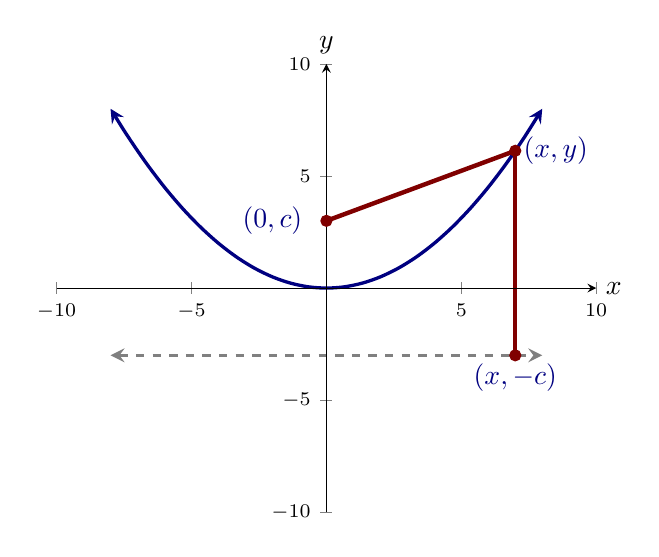
\begin{tikzpicture}
     \begin{axis}[
            	domain=-10:10, ymax=10, xmax=10, ymin=-10, xmin=-10,
            	axis lines =center, xlabel=$x$, ylabel=$y$,
               ytick={-10,-5,5,10},
               xtick={-10,-5,5,10},
               ticklabel style={font=\scriptsize},
            	every axis y label/.style={at=(current axis.above origin),anchor=south},
            	every axis x label/.style={at=(current axis.right of origin),anchor=west},
            	axis on top,
          		]


	
        \addplot[color=penColor2,fill=penColor2,only marks,mark=*] coordinates{(0,3)};
        
        \addplot [draw=penColor, very thick, smooth, domain=(-8:8),<->] {0.125*x^2};
        \addplot [draw=gray, very thick, dashed, domain=(-8:8),<->] {-3};

        \addplot[color=penColor2,fill=penColor2,only marks,mark=*] coordinates{(7,6.125)};
        \addplot[color=penColor2,fill=penColor2,only marks,mark=*] coordinates{(7,-3)};


        




		\node[penColor] at (axis cs:8.5,6.125) {$(x,y)$};
		\node[penColor] at (axis cs:7,-4) {$(x,-c)$};
		\node[penColor] at (axis cs:-2,3) {$(0,c)$};


        \addplot [ultra thick,penColor2] plot coordinates {(7,6.125) (7,-3)};
        \addplot [ultra thick,penColor2] plot coordinates {(7,6.125) (0,3)};
    





    \end{axis}
\end{tikzpicture}
\end{image}


\begin{idea}
If we select a random point, $(x,y)$, on the parabola then the distance from this point to the focus has to equal the distance to the directrix.


\[  \sqrt{x^2 + (y-c)^2} = \answer{y+c}   \]


Simplifying gives


\[  x^2 + (y-c)^2 = (y+c)^2   \]

\[  x^2 + y^2 - \answer{2 y c} + c^2 = y^2 + \answer{2 y c} + c^2   \]

\[  x^2  - 2 y c  =  2 y c    \]

\[  x^2   =  4 y c    \]


The coordinates of the points on the parabola satisfy a quadratic equation.  


\begin{center}
\textbf{\textcolor{red!80!black}{Parabolas are the graphs of quadratic equations!}}
\end{center}


\end{idea}








\subsection*{Projectile Trajectory}


We have descriptions of the vertical height and the horizontal distance for a projectile under the influence of gravity.  Let's put those together and get height as a function of distance.  That will correspond to our normal experience standing on the ground watching a projectile fly.


\begin{itemize}
\item $h_y(t) = s_{y_0} + v_{y_0} t - \frac{9.81}{2} t^2$


\item $d_x(t) = s_{x_0} + v_{x_0} t$
\end{itemize}




First, let's go back to our separate equations and let's just assume we are firing the projectile off the ground.  Then our initial position will be $0$.  

And, let's use the more common symbol $g$, for the acceleration due to gravity, $g = \frac{9.81}{2} \frac{m^2}{s}$, downward.




\begin{itemize}
\item $y = v_{y_0} t - g \, t^2$


\item $x = v_{x_0} t$
\end{itemize}


Solve for $t$ in the horizonal equation.


\[ t = \frac{x}{v_{x_0}} \]

Substitute this into the vertical equation.


\[  y = v_{y_0} \, \frac{x}{v_{x_0}} - g \left(\frac{x}{v_{x_0}}\right)^2  \]



\[  y = \frac{v_{y_0}}{v_{x_0}} \, x  - \frac{g}{(v_{x_0})^2} \, x^2 \]



A quadratic! \\

The projectile itself follows a parabola trajectory in the air. \\


Separately...


The projectile's height is described by a quadratic function in time. \\


The projectile's horizontal distance is not affected by gravity, so it is described by a linear function in time. \\












\begin{center}
\textbf{\textcolor{green!50!black}{ooooo-=-=-=-ooOoo-=-=-=-ooooo}} \\

more examples can be found by following this link\\ \link[More Examples of Quadratics]{https://ximera.osu.edu/csccmathematics/precalculus1/precalculus1/projectileMotion/examples/exampleList}

\end{center}






\end{document}
